% template adapted from https://github.com/jgm/pandoc-templates/blob/master/default.latex

%%% STYLE %%%
\documentclass[12pt,]{article}

%%% PACKAGES %%%

% fonts
\usepackage{lmodern}

% pdf
\usepackage{pdfpages}

% formulae
\usepackage{amssymb,amsmath}
\usepackage{ifxetex,ifluatex}
\usepackage{fixltx2e}
\usepackage[T1]{fontenc}
\usepackage[utf8]{inputenc}

% Tables
% pacakges for kableextra
\usepackage{booktabs}
\usepackage{longtable}
\usepackage{array}
\usepackage{multirow}
\usepackage{wrapfig}
\usepackage{float}
\usepackage{colortbl}
\usepackage{pdflscape}
\usepackage{tabu}
\usepackage{threeparttable}
\usepackage{threeparttablex}
\usepackage[normalem]{ulem}
\usepackage{makecell}
\usepackage{xcolor}
% Fix footnotes in tables (requires footnote package)
\IfFileExists{footnote.sty}{\usepackage{footnote}\makesavenoteenv{long table}}{}

% graphics
\usepackage{graphicx,grffile}
\makeatletter
\def\maxwidth{\ifdim\Gin@nat@width>\linewidth\linewidth\else\Gin@nat@width\fi}
\def\maxheight{\ifdim\Gin@nat@height>\textheight\textheight\else\Gin@nat@height\fi}
\makeatother
\setkeys{Gin}{width=\maxwidth,height=\maxheight,keepaspectratio}

% indent
\IfFileExists{parskip.sty}{%
\usepackage{parskip}
}{% else
\setlength{\parindent}{0pt}
\setlength{\parskip}{6pt plus 2pt minus 1pt}
}

% prevent overfull lines
\setlength{\emergencystretch}{3em}  
\providecommand{\tightlist}{%
\setlength{\itemsep}{0pt}\setlength{\parskip}{0pt}}

\setcounter{secnumdepth}{0}

% set default figure placement to htbp
\makeatletter 
\def\fps@figure{htbp}
\makeatother

% set default table placement to htbp
\makeatletter 
\def\fps@table{htbp}
\makeatother

% code highlights

% hyperlinks
\IfFileExists{upquote.sty}{\usepackage{upquote}}{}
\IfFileExists{microtype.sty}{%
\usepackage[]{microtype}
\UseMicrotypeSet[protrusion]{basicmath} % disable protrusion for tt fonts
}{}
\PassOptionsToPackage{hyphens}{url} % url is loaded by hyperref
\usepackage[unicode=true]{hyperref}
\definecolor{maroon}{cmyk}{0, 0.87, 0.68, 0.32}
\hypersetup{
      pdfborder={0 0 0},
      breaklinks=true}
\urlstyle{same} % don't use monospace font for urls

% geometry
\usepackage[left=2.5cm,right=2.5cm,top=2.5cm,bottom=2.5cm]{geometry}
\renewcommand{\baselinestretch}{1.5}

% Bibliography
\usepackage{natbib}
\bibliographystyle{plainnat}

% SuppMat
\renewcommand{\figurename}{Figure S}
\renewcommand{\tablename}{Table S}
\renewcommand{\contentsname}{Supplemental content}
\renewcommand{\listtablename}{Supplemental tables}
\renewcommand{\listfigurename}{Supplemental figures}

% header
\usepackage[export]{adjustbox}
\usepackage{fancyhdr}
\pagestyle{fancy}
\fancyhead[H]{} 
\renewcommand{\headrulewidth}{0pt}
\renewcommand{\footrulewidth}{0pt}
\setlength\headheight{40.0pt}
\addtolength{\textheight}{-40.0pt}
\chead{
\includegraphics[width=0.2\textwidth,left]{template/newphytologist.png}}

%%% BODY %%%
\begin{document}

\textbf{\emph{New Phytologist} Supporting Information}

Article title: \textbf{Topography drives microgeographic adaptations among closely-related species of two tropical tree species complexes}

Authors: Sylvain Schmitt, Niklas Tysklind, Bruno Hérault, Myriam Heuertz

Article acceptance date: unknown

The following Supporting Information is available for this article:

\textbf{Method S1.} Design of the probes set for \emph{Symphonia}.

\textbf{Method S2.} Design of the probes set for \emph{Eschweilera}.

\textbf{Model S1.} Stan code for the animal model

\textbf{Tab. S\ref{tab:kmeansConfusion}.} \emph{Eschweilera} botanical species and genetic clusters

\textbf{Fig. S\ref{fig:symcapture}.} Target selection for the capture experiment of \emph{Symphonia}

\textbf{Fig. S\ref{fig:parvicapture}.} Target selection for the capture experiment of \emph{Eschweilera}

\textbf{Fig. S\ref{fig:libmiss}.} SNP abundance per library for \emph{Eschweilera}

\textbf{Fig. S\ref{fig:snpmiss}.} Library abundance per SNP for \emph{Eschweilera}

\textbf{Fig. S\ref{fig:outgroup}.} Outgroup detection for \emph{Eschweilera}

\textbf{Fig. S\ref{fig:admixtureSympoCV}.} Cross-validation for \emph{Symphonia} population structure

\textbf{Fig. S\ref{fig:admixtureSympo}.} \emph{Symphonia} population structure using admixture

\textbf{Fig. S\ref{fig:introgress}.} \emph{Symphonia} population structure using hybrid index

\textbf{Fig. S\ref{fig:bayescanOutliers}.} Outlier SNPs among \emph{Symphonia} species

\textbf{Fig. S\ref{fig:conhetero}.} Conspecifics and congenerics in local neighborhood

\newpage

\hypertarget{method-s1-design-of-the-probes-set-for-symphonia.}{%
\section{\texorpdfstring{Method S1: Design of the probes set for \emph{Symphonia}.}{Method S1: Design of the probes set for Symphonia.}}\label{method-s1-design-of-the-probes-set-for-symphonia.}}

For \emph{Symphonia globulifera}, the genomic and transcriptomic resources used for the design were comprised of a published low-coverage draft genome from Africa (Olsson \emph{et al.} \protect\hyperlink{ref-Olsson2017}{2017}), an unpublished draft genome from French Guiana {[}Scotti et al., in prep{]}, an unpublished transcriptome from 20 juveniles from French Guiana {[}Tysklind et al., in prep{]}, and reduced-representation genomic sequence reads of individuals from French Guiana {[}Torroba-Balmori et al., unpublished{]}.
We aligned genomic reads on the two genome drafts with \texttt{bwa} (Li \& Durbin \protect\hyperlink{ref-Li2009}{2009}).
We kept scaffolds from the two genome drafts with a length superior to 1 kbp and at least one matching alignment with a read with a single match on the genome, and merged the two filtered genome drafts with \texttt{quickmerge} (Chakraborty \emph{et al.} \protect\hyperlink{ref-Chakraborty2016}{2016}).
We aligned transcripts on the new filtered genome draft with \texttt{BLAT} (Kent \protect\hyperlink{ref-Kent2002}{2002}) and selected 533 scaffolds without transcript-match, \emph{i.e.} anonymous scaffolds.
We masked repetitive regions with \texttt{RepeatMasker} (Smit \emph{et al.} \protect\hyperlink{ref-Smit2015}{2015}) and selected 533 1-kbp anonymous loci within the 533 previous scaffolds.

Similarly, we filtered transcripts from the 20 juveniles of \emph{Symphonia globulifera} from French Guiana {[}Tysklind et al., in prep{]} based on SNP quality, type and frequency.
We further detected open reading frames (ORFs) using \texttt{transdecoder} (Haas \emph{et al.} \protect\hyperlink{ref-Haas2013}{2013}),
and selected transcripts with non-overlapping ORFs including a start codon.
We kept ORFs with an alignment on scaffolds from the aforementioned genome draft for \emph{Symphonia} using \texttt{BLAT} (Kent \protect\hyperlink{ref-Kent2002}{2002}),
and masked repetitive regions with \texttt{RepeatMasker} (Smit \emph{et al.} \protect\hyperlink{ref-Smit2015}{2015}).
We selected 1,150 genic loci of 500-bp to 1-kbp, from 100 bp before the start to a maximum of 900 bp after the end of the ORFs, resulting in 1-Mbp genomic loci that included a coding region.

\newpage

\hypertarget{method-s2-design-of-the-probes-set-for-eschweilera.}{%
\section{\texorpdfstring{Method S2: Design of the probes set for \emph{Eschweilera}.}{Method S2: Design of the probes set for Eschweilera.}}\label{method-s2-design-of-the-probes-set-for-eschweilera.}}

For \emph{Eschweilera}, the genomic and transcriptomic resources used for the design were comprised of transcriptomes from \emph{Eschweilera sagotiana} and \emph{Eschweilera coriacea} (Vargas \emph{et al.} \protect\hyperlink{ref-Vargas2019}{2019}), and unpublished reduced representation genomic reads (M. Heuertz pers. com.).
We mapped reciprocally \emph{E. coriacea} and \emph{E. sagotiana} transcriptomes using \texttt{BLAT} (Kent \protect\hyperlink{ref-Kent2002}{2002}), and in reciprocal best matches, we kept a single transcript to avoid paralogs and have robust targets among species.
We further detected open reading frames (ORFs) using \texttt{transdecoder} (Haas \emph{et al.} \protect\hyperlink{ref-Haas2013}{2013}),
and selected transcripts with non-overlapping ORFs including a start codon.
We selected 1,530 transcriptomic loci of 500-bp to 1-kbp, from 100 bp before the start to a maximum of 900 bp after the end of the ORFs, resulting in 0.83-Mbp of transcriptomic loci.
To build anonymous targets, we built a \emph{de novo} assembly of ddRAD-seq genomic data using \texttt{ipyrad} (Eaton \& Overcast \protect\hyperlink{ref-Eaton2020}{2020}), mapped consensus sequences on transcripts using \texttt{BLAT} (Kent \protect\hyperlink{ref-Kent2002}{2002}), and kept consensus sequences with no match on transcripts.
We masked repetitive regions with \texttt{RepeatMasker} (Smit \emph{et al.} \protect\hyperlink{ref-Smit2015}{2015}) and selected 2.2k anonymous loci resulting in a length 0.52-Mbp.

\newpage

\hypertarget{references}{%
\section{References}\label{references}}

\hypertarget{refs}{}
\leavevmode\hypertarget{ref-Chakraborty2016}{}%
Chakraborty, M., Baldwin-Brown, J.G., Long, A.D. \& Emerson, J.J. (2016). Contiguous and accurate de novo assembly of metazoan genomes with modest long read coverage. \emph{Nucleic Acids Research}, \textbf{44}, 1--12.

\leavevmode\hypertarget{ref-Eaton2020}{}%
Eaton, D.A.R. \& Overcast, I. (2020). ipyrad: Interactive assembly and analysis of RADseq datasets. \emph{Bioinformatics (Oxford, England)}, \textbf{36}, 2592--2594.

\leavevmode\hypertarget{ref-Haas2013}{}%
Haas, B.J., Papanicolaou, A., Yassour, M., Grabherr, M., Philip, D., Bowden, J., Couger, M.B., Eccles, D., Li, B., Macmanes, M.D., Ott, M., Orvis, J., Pochet, N., Strozzi, F., Weeks, N., Westerman, R., William, T., Dewey, C.N., Henschel, R., Leduc, R.D., Friedman, N. \& Regev, A. (2013). \emph{De novo transcript sequence recostruction from RNA-Seq: reference generation and analysis with Trinity}.

\leavevmode\hypertarget{ref-Kent2002}{}%
Kent, W.J. (2002). BLAT---The BLAST-Like Alignment Tool. \emph{Genome Research}, \textbf{12}, 656--664.

\leavevmode\hypertarget{ref-Li2009}{}%
Li, H. \& Durbin, R. (2009). Fast and accurate short read alignment with Burrows-Wheeler transform. \emph{Bioinformatics}, \textbf{25}, 1754--1760.

\leavevmode\hypertarget{ref-Olsson2017}{}%
Olsson, S., Seoane-Zonjic, P., Bautista, R., Claros, M.G., González-Martínez, S.C., Scotti, I., Scotti-Saintagne, C., Hardy, O.J. \& Heuertz, M. (2017). Development of genomic tools in a widespread tropical tree, Symphonia globulifera L.f.: a new low-coverage draft genome, SNP and SSR markers. \emph{Molecular Ecology Resources}, \textbf{17}, 614--630. Retrieved from \url{http://doi.wiley.com/10.1111/1755-0998.12605}

\leavevmode\hypertarget{ref-Smit2015}{}%
Smit, A., Hubley, R. \& Green, P. (2015). RepeatMasker Open-4.0. \textless http://www.repeatmasker.org\textgreater.

\leavevmode\hypertarget{ref-Vargas2019}{}%
Vargas, O.M., Heuertz, M., Smith, S.A. \& Dick, C.W. (2019). Target sequence capture in the Brazil nut family (Lecythidaceae): Marker selection and in silico capture from genome skimming data. \emph{Molecular Phylogenetics and Evolution}, \textbf{135}, 98--104. Retrieved from \url{https://www.sciencedirect.com/science/article/pii/S1055790318304895}

\newpage

\hypertarget{model-s1-stan-code-for-the-bayesian-inference-of-the-animal-model.}{%
\section{Model S1: Stan code for the bayesian inference of the animal model.}\label{model-s1-stan-code-for-the-bayesian-inference-of-the-animal-model.}}

\begin{verbatim}
data {
  int<lower=0>  N ; // # of individuals
  int<lower=0>  P ; // # of populations
  real y[N] ; // phenotype
  int<lower=1, upper=P> population[N] ; // populations
  cov_matrix[N] K ; // kinship covariance matrix
}
transformed data{
  matrix[N, N] A = cholesky_decompose(K) ; // cholesky-decomposed kinship
  real Vy = variance(log(y)) ;
}
parameters {
  vector<lower=0>[P] mu ; // intercept
  vector[N] epsilon ; // genotypic noise
  real<lower=0, upper=sqrt(Vy)> sigma ; // genetic variance
}
transformed parameters {
  real<lower=0> Vp = variance(log(mu[population])) ; // population variance
  real Vr = square(sigma) ;
  real Vg = Vy - Vp - Vr ;
  vector[N] alog = sqrt(Vg)*A*epsilon ;
}
model {
  y ~ lognormal(log(mu[population]) + alog, sigma) ;
  epsilon ~ std_normal() ;
  mu ~ lognormal(0, 1) ;
  sigma ~ normal(0, 1) ;
}
\end{verbatim}

\newpage

\begin{longtable}[]{@{}lrrr@{}}
\caption{\label{tab:kmeansConfusion}Confusion matrix (percentage) between genetic species and botanical identification for \emph{Eschweilera} clade \emph{Parvifolia}.}\tabularnewline
\toprule
Species & E. coriacea cluster & E. decolorans cluster & E. sagotiana cluster\tabularnewline
\midrule
\endfirsthead
\toprule
Species & E. coriacea cluster & E. decolorans cluster & E. sagotiana cluster\tabularnewline
\midrule
\endhead
E. coriacea & 65 & 8 & 13\tabularnewline
E. decolorans & 15 & 77 & 7\tabularnewline
E. sagotiana & 20 & 16 & 80\tabularnewline
\bottomrule
\end{longtable}

\newpage

\begin{figure}[H]

{\centering 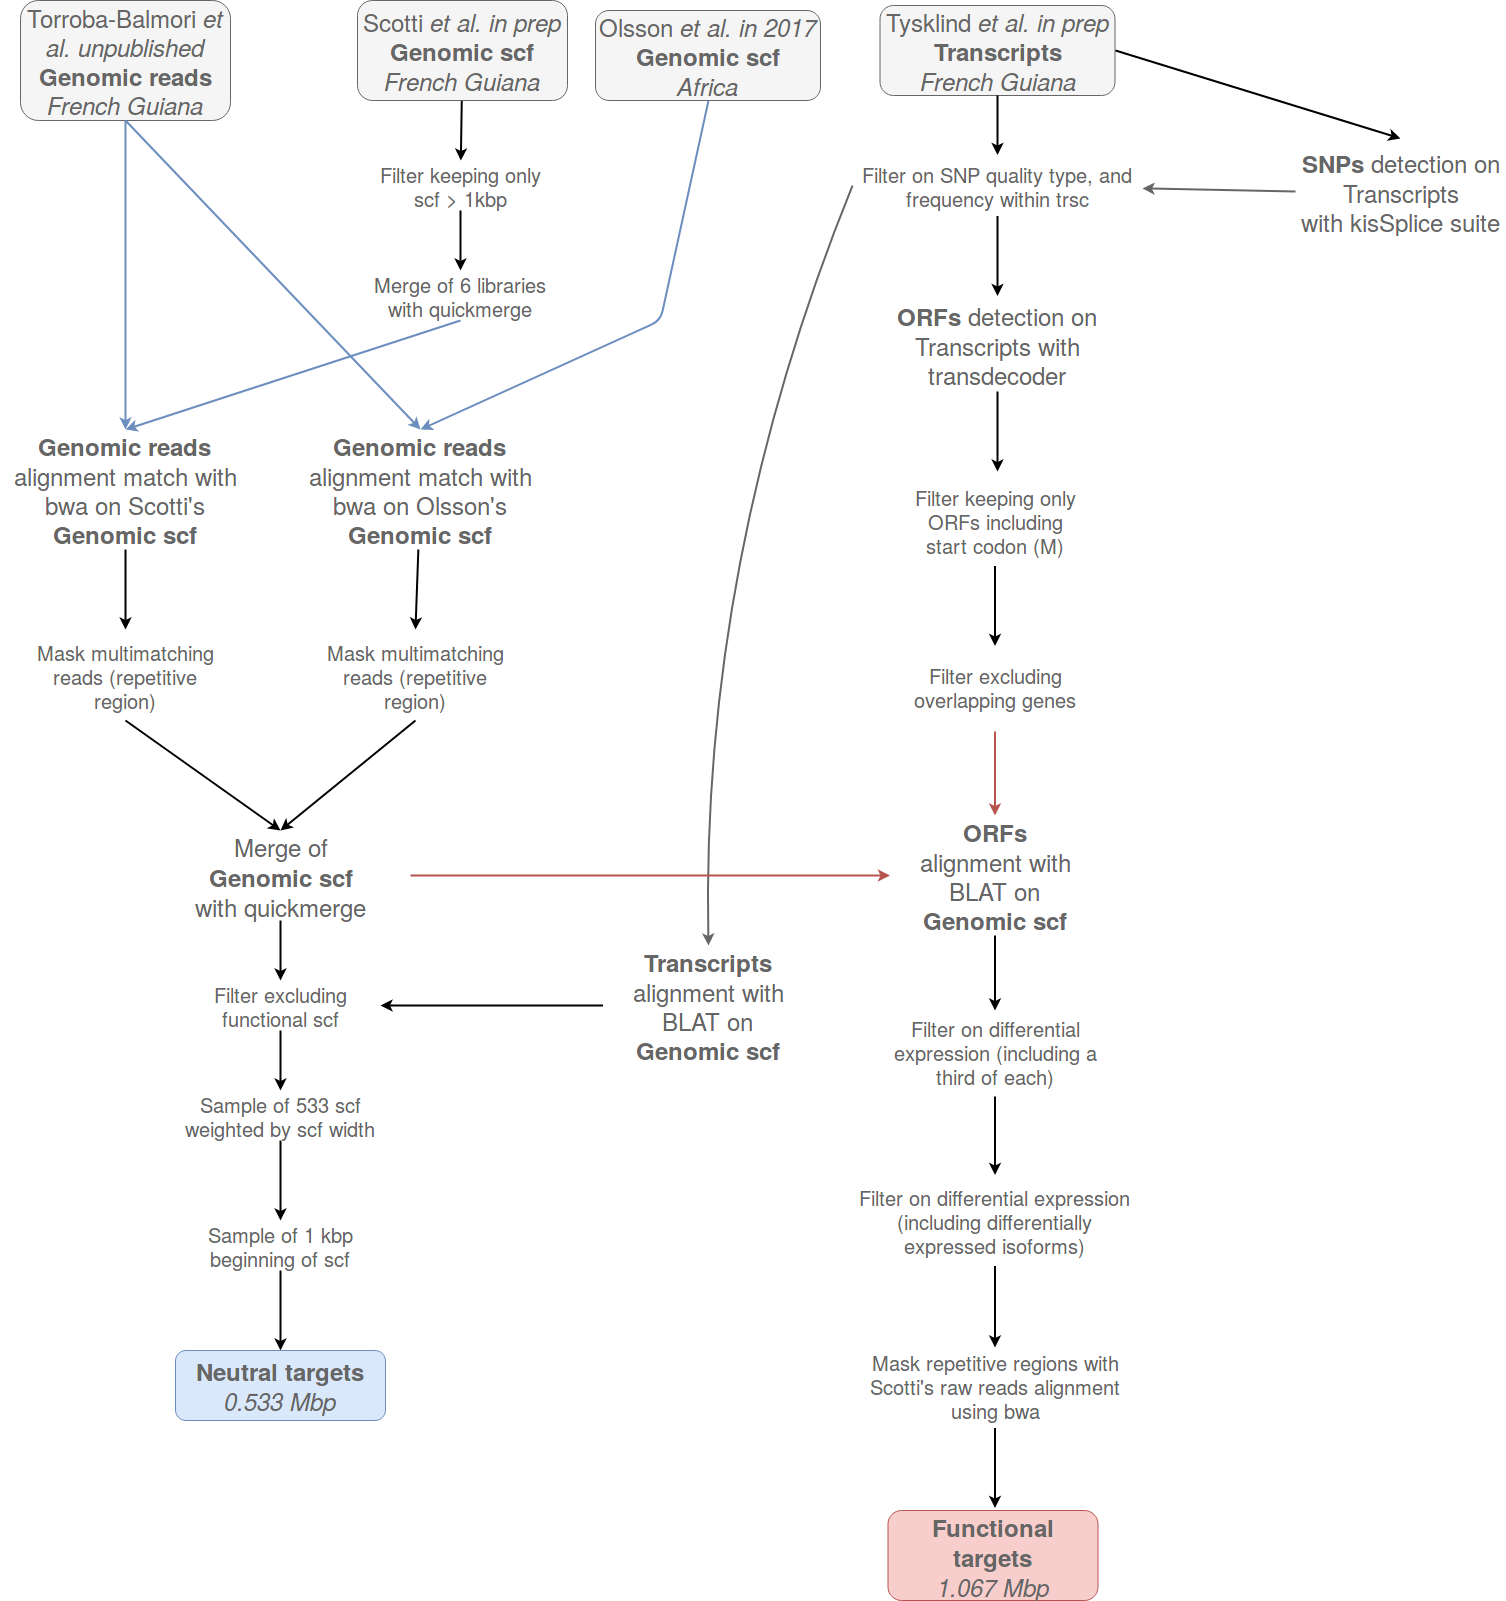
\includegraphics[width=\linewidth]{figures/Symcapture} 

}

\caption{Scheme of target selection for the capture experiment of \emph{Symphonia globulifera} as described in the manuscript.}\label{fig:symcapture}
\end{figure}

\newpage

\begin{figure}[H]

{\centering 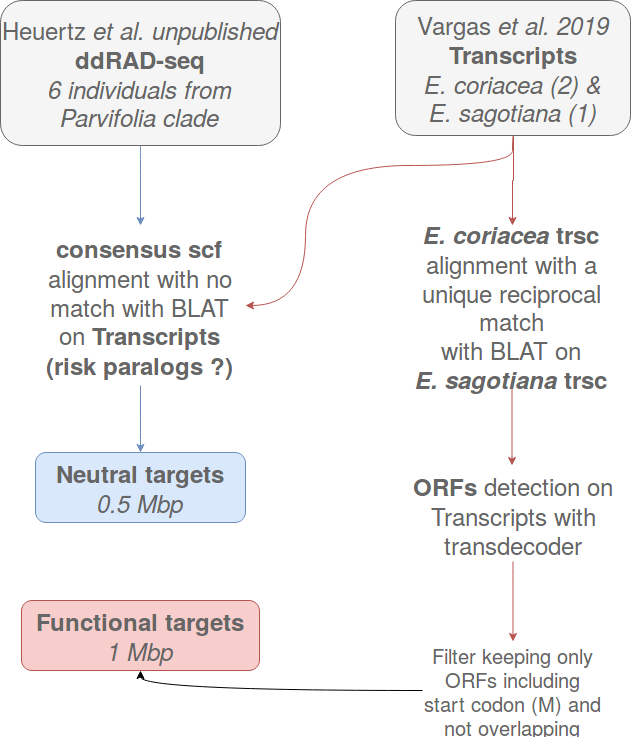
\includegraphics[width=0.5\linewidth]{figures/Parvicapture} 

}

\caption{Scheme of target selection for the capture experiment of \emph{Eschweilera} clade \emph{Parvifolia} as described in the manuscript.}\label{fig:parvicapture}
\end{figure}

\newpage

\begin{figure}[H]

{\centering \includegraphics{TopoSINewPhyto_files/figure-latex/libmiss-1} 

}

\caption{SNP abundance per library rank for raw data of \emph{Eschweilera} clade \emph{Parvifolia}. Dashed lines represent tested filters.}\label{fig:libmiss}
\end{figure}

\newpage

\begin{figure}[H]

{\centering \includegraphics{TopoSINewPhyto_files/figure-latex/snpmiss-1} 

}

\caption{Library abundance per SNP rank for library-filtered data of \emph{Eschweilera} clade \emph{Parvifolia}. Dashed lines represent tested filters.}\label{fig:snpmiss}
\end{figure}

\newpage

\begin{figure}
\centering
\includegraphics{TopoSINewPhyto_files/figure-latex/outgroup-1.pdf}
\caption{\label{fig:outgroup}Outgroup detection with \emph{Eschweilera} individual clustering in the genomic principal component analysis (gPCA) in two groups using K-means for every filter.}
\end{figure}

\newpage

\begin{figure}
\centering
\includegraphics{TopoSINewPhyto_files/figure-latex/admixtureSympoCV-1.pdf}
\caption{\label{fig:admixtureSympoCV}Cross-validation for the clustering of \emph{Symphonia} individuals using admixture. Y axis indicates cross-validation mean error, suggesting that K = 2 or K = 3 gene pools represent the best solution for genetic structure in \emph{Symphonia} in Paracou.}
\end{figure}

\newpage

\begin{figure}
\centering
\includegraphics{TopoSINewPhyto_files/figure-latex/admixtureSympo-1.pdf}
\caption{\label{fig:admixtureSympo}Population structure of \emph{Symphonia} individuals from K=2 to K=10 using admixture.}
\end{figure}

\newpage

\begin{figure}
\centering
\includegraphics{TopoSINewPhyto_files/figure-latex/introgress-1.pdf}
\caption{\label{fig:introgress}Genotypinc constitution of \emph{Symphonia} using hybrid index. Admixture coefficients (black line) are given with 90\% confidence interval (light shade). Admixture coefficients of 10 and 90\% are indicated by white stippled lines.}
\end{figure}

\newpage

\begin{figure}
\centering
\includegraphics{TopoSINewPhyto_files/figure-latex/bayescanOutliers-1.pdf}
\caption{\label{fig:bayescanOutliers}High-differentiation outlier SNPs for \emph{Symphonia} individuals detected with bayescan. We used the genome-transcriptome alignments built for the design of probes sets (Method S1) to classify called SNPs into (i) anonymous SNPs (on scaffolds matching no transcripts), (ii) putatively-hitchhiker SNPs (close to a transcript or within an intron), and (iii) genic SNPs (within an exon).}
\end{figure}

\newpage

\begin{figure}
\centering
\includegraphics{TopoSINewPhyto_files/figure-latex/conhetero-1.pdf}
\caption{\label{fig:conhetero}The relationship between the number of conspecific and congeneric individuals in a local neighborhood with 25 m radius around trees from Symphonia and Eschweilera clade Parvifolia. Each point represents the mean values for all individuals in Paracou, and thin lines the standard deviation.The solid line illustrates a 1:1 ratio.}
\end{figure}

\newpage

\begin{longtable}[]{@{}lrrr@{}}
\caption{\label{tab:blindIdentification}Confusion matrix (count) between genetic species and second blind-identification of individual morphotypes for \emph{Symphonia}.}\tabularnewline
\toprule
Species & S .sp.1 morphotype & S .sp.2 morphotype & S .sp.3 morphotype\tabularnewline
\midrule
\endfirsthead
\toprule
Species & S .sp.1 morphotype & S .sp.2 morphotype & S .sp.3 morphotype\tabularnewline
\midrule
\endhead
S. sp.1 & 28 & 6 & 0\tabularnewline
S. sp.2 & 0 & 11 & 0\tabularnewline
S. sp.3 & 0 & 0 & 21\tabularnewline
\bottomrule
\end{longtable}

\newpage

\begin{figure}
\centering
\includegraphics{TopoSINewPhyto_files/figure-latex/gnomFrac-1.pdf}
\caption{\label{fig:gnomFrac}Distribution of derived or minor allele among species from \emph{Symphonia} and \emph{Eschweilera} clade \emph{Parvifolia}. For \emph{Symphonia}, count and percentage represent the number of derived alleles within and among american species compared to the african reference from Olsson \emph{et al.} (\protect\hyperlink{ref-Olsson2017}{2017}). For \emph{Eschweilera}, count and percentage represent the number of minor alleles within and among species because of the de novo reference.}
\end{figure}

\end{document}
